% =====================================================================
%  PTorch -- Master's thesis defense  (FIGMA / PITCH-STYLE RESTYLE)
%  Jeff Cyuzuzo Jambe
%
%  Look: soft sage canvas, ink-black type, single emerald accent, big
%  bold left-aligned frametitles, white rounded cards, full-bleed black
%  section dividers.
%  Same content + figure paths as the original deck.
%
%  Compile: pdflatex presentation.tex   (run TWICE for n/N to settle).
%  Fonts:   Montserrat (text, pdflatex-safe) + Latin Modern (math).
%
%  SWAPS:
%   - KU Leuven brand instead of green?
%     set SPRING/SPRINGDK to KUL blue,
%     INK stays, SAGE -> very light grey. One block below.
%   - Pixel-closer font (Inter/Aktiv feel)? compile with lualatex and
%     replace the font block with fontspec + \setsansfont{Inter}.
% =====================================================================
\documentclass[aspectratio=169,10pt]{beamer}

\usetheme{default}
\usecolortheme{default}
\setbeamertemplate{navigation symbols}{}

\usepackage[utf8]{inputenc}
\usepackage[T1]{fontenc}
\usepackage{lmodern}                 % scalable Latin Modern -> used for MATH
\usepackage{montserrat}              % Montserrat -> used for all TEXT (pdflatex)
\renewcommand{\familydefault}{\sfdefault}
\usepackage[tracking=true]{microtype}
\usepackage{mathrsfs}
\usepackage{amsmath,amssymb,amsfonts,mathtools}
\usepackage{bbm}
\usepackage{graphicx}
\usepackage{booktabs}
\usepackage{tikz}
\usepackage{xcolor}
\usepackage{listings}
\usepackage{adjustbox}

\usetikzlibrary{arrows.meta,positioning,fit,backgrounds,calc}

\DeclareMathOperator*{\minimize}{minimize}
\DeclareMathOperator*{\argmin}{arg\,min}
\DeclareMathOperator{\prox}{prox}
\newcommand{\dist}{\operatorname{dist}}
\newcommand{\PT}{\ensuremath{\mathcal{P}}Torch}

% ---- PALETTE (KU Leuven huisstijl) --------------------------------
%  Source: https://associatie.kuleuven.be/huisstijl/kleuren
%   primary navy 00407A, light blue 52BDEC, medium blue 1FABD5,
%   deep blue 116E8A, accent orange DD8A2E.
\definecolor{INK}{RGB}{14,16,15}        % near-black text & full-bleed slides
\definecolor{SAGE}{RGB}{238,244,249}    % very light blue-grey canvas
\definecolor{SPRING}{RGB}{82,189,236}   % KUL light blue accent (fills, blocks)
\definecolor{SPRINGDK}{RGB}{0,64,122}   % KUL primary navy (text/emphasis on light)
\definecolor{MUT}{RGB}{120,131,140}     % muted blue-grey (footer, captions)
\definecolor{CARD}{RGB}{255,255,255}
% white card
\definecolor{HAIR}{RGB}{205,216,226}    % hairline border (cool grey)
\definecolor{CODEBG}{RGB}{255,255,255}
\definecolor{CODEKW}{RGB}{0,64,122}
\definecolor{CODECM}{RGB}{120,131,140}
\definecolor{KULORANGE}{RGB}{221,138,46} % KUL accent orange (sparingly)

\setbeamercolor{background canvas}{bg=SAGE}
\setbeamercolor{normal text}{fg=INK,bg=SAGE}
\setbeamercolor{structure}{fg=SPRINGDK}
\setbeamercolor{alerted text}{fg=SPRINGDK}
\setbeamercolor{title}{fg=INK}
\setbeamercolor{frametitle}{fg=INK,bg=}
\setbeamerfont{frametitle}{size=\LARGE,series=\bfseries}
\setbeamerfont{title}{series=\bfseries}

% rounded white blocks with an emerald title bar
\setbeamertemplate{blocks}[rounded][shadow=false]
\setbeamercolor{block title}{fg=INK,bg=SPRING}
\setbeamercolor{block body}{fg=INK,bg=CARD}

\newcommand{\spaced}[1]{\textls[120]{\MakeUppercase{#1}}}

% ---- frametitle: bold, top-left, generous margin, no bar ----------
\setbeamertemplate{frametitle}{%
  \vskip14pt%
  \hspace{20pt}{\usebeamerfont{frametitle}\color{INK}\insertframetitle}%
  \vskip4pt%
}

% ---- footline: quiet, uppercase, letter-spaced --------------------
\newcommand{\footmid}{\insertsectionhead}
\setbeamertemplate{footline}{%
  \leavevmode%
  \hbox{\hspace{20pt}%
    {\scriptsize\color{MUT}\spaced{PTorch}}%
    \hfill
    {\scriptsize\color{MUT}\spaced{\footmid}}%
    \hfill
    {\scriptsize\color{MUT}\insertframenumber\,/\,\inserttotalframenumber}%
    \hspace{20pt}}%
  \vskip9pt%
}

% ---- bullets: small emerald squares -------------------------------
\setbeamertemplate{itemize item}{\textcolor{SPRING}{\rule[0.18ex]{0.72ex}{0.72ex}}}
\setbeamertemplate{itemize subitem}{\textcolor{INK}{\rule[0.18ex]{0.5ex}{0.5ex}}}
\setbeamertemplate{enumerate item}{\color{SPRINGDK}\bfseries\insertenumlabel.}

% ---- robust figure include ----------------------------------------
\newcommand{\safeincludegraphics}[2][width=\linewidth]{%
  \IfFileExists{#2}{\includegraphics[#1]{#2}}%
  {\fcolorbox{SPRINGDK}{SPRING!8}{\parbox[c][0.42\textheight][c]{0.9\linewidth}{\centering\small\ttfamily missing: #2}}}%
}

% ---- white rounded card (figma) -----------------------------------
\newcommand{\card}[1]{%
  \begin{center}%
  \begin{tikzpicture}%
    \node[fill=CARD,draw=HAIR,line width=0.6pt,rounded corners=8pt,
          inner sep=12pt,text width=0.88\linewidth,align=center] {#1};%
  \end{tikzpicture}%
  \end{center}}

% ---- emerald emphasis card (use for the real punchlines) ----------
\newcommand{\keycard}[1]{%
  \begin{center}%
  \begin{tikzpicture}%
    \node[fill=SPRING,rounded corners=8pt,inner sep=12pt,text=INK,
          text width=0.88\linewidth,align=center] {#1};%
  \end{tikzpicture}%
  \end{center}}

% ---- figure card: white rounded frame + muted caption -------------
\newcommand{\figcard}[3][width=\linewidth]{%
  \begin{center}%
  \begin{tikzpicture}%
    \node[fill=CARD,draw=HAIR,line width=0.6pt,rounded corners=6pt,inner sep=6pt]
      {\safeincludegraphics[#1]{#2}};%
  \end{tikzpicture}\\[0.3em]%
  {\footnotesize\color{MUT}#3}%
  \end{center}}

% ---- python listing style (white code card) -----------------------
\lstdefinestyle{py}{
  language=Python,
  basicstyle=\ttfamily\scriptsize\color{INK},
  backgroundcolor=\color{CODEBG},
  keywordstyle=\color{CODEKW}\bfseries,
  commentstyle=\color{CODECM}\itshape,
  stringstyle=\color{INK},
  showstringspaces=false,
  breaklines=true,
  frame=single,
  framesep=8pt,
  rulecolor=\color{HAIR},
  xleftmargin=2pt,xrightmargin=2pt,
  aboveskip=4pt,belowskip=4pt,
  escapeinside={(*@}{@*)},
}

% ---- section divider: full-bleed black, big emerald accent --------
\AtBeginSection[]{%
  {\setbeamercolor{background canvas}{bg=INK}%
  \begin{frame}[plain]
    \vfill
    \hspace{24pt}{\color{SPRING}\rule{42pt}{4pt}}\par
    \vskip16pt
    \hspace{24pt}{\usebeamerfont{frametitle}\color{white}\Huge\insertsectionhead}\par
    \vfill
  \end{frame}}%
}

% -------------------------------------------------------------------
\title{$\mathcal{P}$Torch}
\subtitle{Narrowing the Gap Between Projection-- and Gradient--Based Learning}
\author{Jeff Cyuzuzo Jamb\'e}

\begin{document}

% ============================== TITLE ==============================
\begin{frame}[plain]
  % KU Leuven logo, flush top-right (needs a 2nd pdflatex pass to settle)
  \begin{tikzpicture}[remember picture,overlay]
    \node[anchor=north east]
      at ([xshift=-24pt,yshift=-20pt]current page.north east)
      {
\includegraphics[height=34pt]{image.png}};
  \end{tikzpicture}
  \vspace{34pt}
  \hspace{24pt}\begin{minipage}{0.92\textwidth}
    {\color{SPRINGDK}\footnotesize\spaced{Master's Thesis \;\textbullet\; Artificial Intelligence \;\textbullet\; KU Leuven}}\par
    \vskip22pt
    {\fontsize{58}{60}\selectfont\mdseries\color{INK}{\color{SPRINGDK}$\mathcal{P}$}Torch}\par
    \vskip12pt
        {\LARGE\color{INK}Narrowing the Gap Between\\[2pt]Projection and Gradient Based Learning}\par
    \vskip30pt
    {\footnotesize\color{MUT}%
      Author: Jeff Cyuzuzo Jamb\'e\\[2pt]
      Promotor: Prof.\,dr.\,ir.\,Panos Patrinos\\[1pt]
      Assessors: Prof.\,dr.\,ir.\,Raf Vandebril \;\textbar\; Prof.\,dr.\,ir.\,Matthew Blaschko\\[1pt]
      Supervisor: Ir.\,Jan Quan}
  \end{minipage}
\end{frame}

% ===================================================================
\section{Motivation}
% ===================================================================
\begin{frame}[fragile]{Paradigm lock-in}
  Modern neural networks rely on two lines:
  
  \vspace{1em}
  \begin{lstlisting}[style=py]
loss = criterion(model(x), y)
loss.backward()  # Global credit assignment
  \end{lstlisting}

  \vfill
  \begin{itemize}
    \item \textbf{Requirement:} Every component must be differentiable.
    \item \textbf{Risk:} \alert{Paradigm lock-in} — alternatives stay under-explored.
  \end{itemize}

  \vfill
  \centering
  \large\color{INK}
  \textbf{What if \texttt{backward()} computed something else?}
\end{frame}

\begin{frame}{Learning as a feasibility problem}
  Search for a point in the
  \alert{intersection of constraint sets}.
  \vspace{0.3em}
  \card{$\displaystyle
  \minimize_{\theta\in\Theta}\ \mathcal{L}\bigl(f(x;\theta),y\bigr)
  \quad\rightarrow\quad
  \text{find } \tilde\theta \in \bigcap_{i=1}^{m} C_i$}
  \vspace{0.3em}
  \begin{itemize}
    \item $\tilde\theta$ \alert{perfectly interpolate}
          the data
    \item Solved with \alert{cyclic / averaged projections,
          Douglas--Rachford,...}
    \item \alert{severe memory cost}, far slower.
  \end{itemize}
\end{frame}

\begin{frame}{Research question}
  \vspace{1.5em}
  \begin{minipage}{0.9\linewidth}
    {\large\color{INK}
    Can we design a projection-based training framework native to modern
    deep-learning toolchains that eliminates severe memory bottlenecks, avoids
    computational overhead, and achieves performance competitive with
    gradient-based methods?}
  \end{minipage}

  \vfill
  
  {\small\color{MUT}\spaced{This talk's spine}}\\[0.5em]
  \begin{itemize}
    \setlength{\itemsep}{0.4em}
    \item The autograd backward pass as cyclic projections.
    \item The projection residual is a genuine gradient.
    \item optimizers (Adam, Muon) become a nonlinear relaxations.
  \end{itemize}
  \vspace{1em}
\end{frame}

% ===================================================================
\section{The idea}
% ===================================================================
\begin{frame}{A network is a stack of interlocking constraints}
  \vspace{1em}
  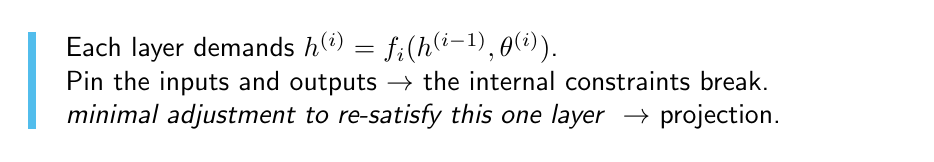
\begin{tikzpicture}
    \node[inner sep=0pt, right] (text) at (0,0) {
      \begin{minipage}{0.88\linewidth}
        Each layer demands $h^{(i)}=f_i(h^{(i-1)},\theta^{(i)})$.\\
        Pin the inputs and outputs $\rightarrow$ the internal constraints break.\\
        \textit{minimal adjustment to re-satisfy this one layer}\; $\rightarrow$ \alert{projection}.
      \end{minipage}
    };
    \draw[SPRING, line width=3pt] ([xshift=-12pt]text.north west) -- ([xshift=-12pt]text.south west);
  \end{tikzpicture}

  \vfill
  
  {\small\color{MUT}\spaced{Find $\omega$ in the intersection of 3 constraints:}}\par\vspace{0.8em}
  \begin{description}
    \setlength{\itemsep}{0.6em}
    \item[{\color{SPRINGDK}A}rchitectural] $h_b^{(i)}=f_i(h_b^{(i-1)},\theta_b^{(i)})$ \hfill {\footnotesize\color{MUT}(layer obeys map)}
    \item[{\color{SPRINGDK}B}atch (data)] $h_b^{(0)}=x_b,\ h_b^{(N)}=y_b$ \hfill {\footnotesize\color{MUT}(ends pinned)}
    \item[{\color{SPRINGDK}C}onsensus] $\theta_1^{(i)}=\dots=\theta_B^{(i)}$ \hfill {\footnotesize\color{MUT}(average over batch)}
  \end{description}
  \vspace{0.5em}
\end{frame}

\begin{frame}{Intuition: XOR as a feasibility problem}
  \begin{columns}[T,onlytextwidth]
    \begin{column}{0.52\textwidth}
      \vspace{0.5em}
      \begin{itemize}
        \item XOR: simple, but \alert{not linearly separable}.
        \item Each datapoint $\to$ a feasible \alert{slice} ($A_{b3}\cap B_{\mathrm{out}}$).
        \item Consensus ties the per-sample copies together.
      \end{itemize}
      \vspace{0.4em}
      \card{The \alert{green} intersection $\rightarrow$ perfect interpolation.}
    \end{column}
    \begin{column}{0.4\textwidth}
        \centering
        
         \input{xor_pres}
    \end{column}
  \end{columns}
\end{frame}

\begin{frame}{The key idea: backward pass $=$ cyclic projection}
  \begin{itemize}
    \item Forward pass is \alert{identical} to standard training.
    \item Backward computes a \alert{projection target}, not a gradient.
  \end{itemize}

  \vspace{-0.5em}
  \begin{center}
  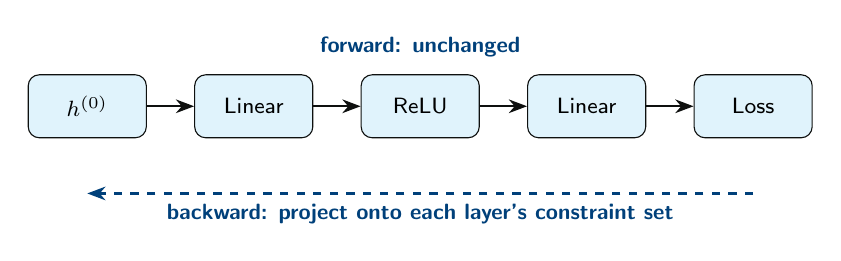
\begin{tikzpicture}[font=\footnotesize,>=Stealth,node distance=6mm]
    \tikzset{op/.style={draw=INK,rounded corners,minimum height=8mm,minimum width=15mm,fill=SPRING!18}}
    \node[op] (x) {$h^{(0)}$};
    \node[op,right=of x] (l1) {Linear};
    \node[op,right=of l1] (a) {ReLU};
    \node[op,right=of a] (l2) {Linear};
    \node[op,right=of l2] (loss) {Loss};
    \draw[->,INK,thick] (x)--(l1); \draw[->,INK,thick] (l1)--(a);
    \draw[->,INK,thick] (a)--(l2); \draw[->,INK,thick] (l2)--(loss);
    \node[above=1mm of a,SPRINGDK] {\textbf{forward: unchanged}};
    \draw[->,SPRINGDK,thick,dashed] ([yshift=-7mm]loss.south)--([yshift=-7mm]x.south)
      node[midway,below,SPRINGDK]{\textbf{backward: project onto each layer's constraint set}};
  \end{tikzpicture}
  \end{center}
\end{frame}

\begin{frame}{The residual is a gradient}
  The feasibility problem equals $\minimize_\omega F(\omega)=\sum_j f_j(\omega)$
  with $f_j=\tfrac12\dist^2(\tilde C_j,\cdot)$. Wherever the projection is
  single-valued,
  \[
  \nabla f_j(\omega)=\omega-\Pi_{\tilde C_j}(\omega)
  \qquad(\text{exactly the projection \alert{residual}}).
  \]
  So a plain projection step is an \alert{incremental gradient step}:
  \[
  \bar\theta\gets\theta-\alpha\bigl(\theta-\Pi_{\tilde C_j}(\theta)\bigr)
  =\theta-\alpha\,\nabla f_j(\theta).
  \]
  \begin{block}{Nonlinear relaxation}
  In \PT{} the residual populates \texttt{.grad}. \alert{Adam and Muon }
  using projection targets as adaptive, nonlinear relaxations.
  \end{block}
\end{frame}

% ---- DEMO ---------------------------------------------------------
\begin{frame}[fragile]{Demo: a near drop-in replacement for PyTorch}
  \begin{columns}[T,onlytextwidth]
    \begin{column}{0.5\textwidth}
      \centering\textbf{Standard PyTorch}
      \begin{lstlisting}[style=py]
import torch.nn as nn
import torch.optim as optim

model     = nn.Linear(784, 10)
criterion = nn.CrossEntropyLoss()
optimizer = optim.SGD(model.parameters(),
                      lr=1.0)

logits = model(x)
criterion(logits, y).backward()
optimizer.step()
      \end{lstlisting}
    \end{column}
    \begin{column}{0.5\textwidth}
      \centering\textbf{\color{SPRINGDK}\PT}
      \begin{lstlisting}[style=py]
import ptorch                       (*@\textcolor{SPRINGDK}{\# overrides torch}@*)
import ptorch.nn.modules as pnn
import ptorch.optim_static as poptim

model     = pnn.Linear(784, 10)
criterion = pnn.CrossEntropy()
optimizer = poptim.ProjectionSGD(
                model.parameters(), lr=1.0)

logits = model(x)
criterion(logits, y).sum().backward() (*@\textcolor{SPRINGDK}{\# = projection!}@*)
optimizer.step()
      \end{lstlisting}
    \end{column}
  \end{columns}
  \vspace{-1em}
  \begin{center}\footnotesize
  Same training loop, swapped imports. \quad\textbf{Live:}\;
  \texttt{python -m experiments.mlp.bench\_ptorch -{}-max-steps 50 -{}-num-runs 1}
  \end{center}
\end{frame}

% ===================================================================
\section{Making it practical}
% ===================================================================
\begin{frame}{Fused projections}
  \textbf{Problem.} linear layer projection  builds
  $N_{\mathrm{in}}\times N_{\mathrm{out}}\times B$ tensor
  \begin{quote}\footnotesize\itshape\color{MUT}
  ``the high memory demands of the 4-layer CNN necessitated reducing the hidden
  units to 16 to fit within 96\,GB GPU memory'' --- PJAX
  \end{quote}
  \textbf{Idea.} Projection composition is associative $\Rightarrow$ \alert{fuse} the
  bilinear (architectural) and consensus projections into one matrix multiply ---
  no 3-D tensor is ever formed:
  \[
  \bar\theta^{(i)}=\tfrac1B\bigl(\theta^{(i)}\odot(U\mathbf{1})+VH\bigr).
  \]
  \keycard{Peak memory: $\mathcal{O}(N_{\mathrm{in}}N_{\mathrm{out}}B)\;\to\;
  \mathcal{O}(N_{\mathrm{in}}B+N_{\mathrm{out}}B+N_{\mathrm{in}}N_{\mathrm{out}})$.}
  \footnotesize We then train a 32-64-128 CNN, a ResNet-8, and 2048-filter CNNs. A heavier $\ell_\infty$ variant gives better per-step accuracy
  $\Rightarrow$ \alert{mix and match} ($\ell_2$ for big shared layers,
  $\ell_\infty$ elsewhere). \emph{(derivation in backup)}
\end{frame}

\begin{frame}{Proximal projection at the loss}
  The rigid target snap $h^{(N)}\!\gets y$ is one extreme. Replace it by the
  \alert{proximal operator} of the loss:
  \[
  h^{(N)}\gets\prox_{\lambda\mathcal{L}(\cdot,y)}(h^{(N)})
  =\argmin_u\Bigl\{\mathcal{L}(u,y)+\tfrac{1}{2\lambda}\|u-h^{(N)}\|^2\Bigr\}.
  \]
  \begin{itemize}
    \item Exactly one gradient step on the \alert{Moreau envelope}
          $\mathcal{L}_\lambda$; the rigid snap is the $\lambda\!\to\!0$ limit.
    \item Same minimizers (convex $\mathcal{L}$), but a \alert{bounded backward
          signal} --- for MSE the residual contracts by $\tfrac{1}{1+\lambda}$.
  \end{itemize}
  \card{Now \alert{every} constraint --- including the loss --- is a single
  differentiable gradient step. Cleaner theory, better stability.}
  \footnotesize And the mini-batch loop fixes $K=1$ (one backward sweep per batch)
  $\Rightarrow$ a near drop-in replacement for standard PyTorch training.
\end{frame}

% ===================================================================
\section{The limit, and the evidence}
% ===================================================================
\begin{frame}{Vanishing targets}
  Define the per-layer target magnitude
  $\delta^{(i)}:=\|\bar h^{(i)}-h^{(i)}\|_2$.
  \begin{block}{Theorem (informal)}
  Under local non-expansiveness of the layer projection, for cyclic projections
  \[
  \delta^{(0)}\le\delta^{(1)}\le\dots\le\delta^{(N)}<\infty,
  \]
  \emph{strictly} decreasing wherever a layer is actively learning
  ($\|\Delta\theta^{(i+1)}\|_2>0$).
  \end{block}
    \begin{itemize}
        \item early layers decays with depth
        \item analogue of the \alert{vanishing-gradient} problem

    \end{itemize}
\end{frame}

\begin{frame}{Shallow MLP: competitive with gradient descent}
  \footnotesize One hidden layer, 512 ReLU units. Baselines: Torch (gradient), PJAX (projection).
  \begin{columns}[c,onlytextwidth]
    \begin{column}{0.5\textwidth}
      \figcard[width=0.9\linewidth,height=0.45\textheight,keepaspectratio]{images/mlp/CIFAR10_1L_STEP.pdf}{CIFAR-10: accuracy vs.\ step}
    \end{column}
    \begin{column}{0.5\textwidth}
      \figcard[width=0.9\linewidth,height=0.45\textheight,keepaspectratio]{images/mlp/MNIST_1L_STEP.pdf}{MNIST: accuracy vs.\ step}
    \end{column}
  \end{columns}
\end{frame}

\begin{frame}{Depth degrades projection-based training}
    \figcard[width=0.8\linewidth,height=0.45\textheight,keepaspectratio]{images/deep/vanishing_combined.pdf}
        {$\delta_k$ decays away from the output; MSE worsens with depth.}
  \vspace{0.1em}
  \begin{itemize}
    \item\footnotesize Identity-recovery: layers $\geq3$ from the output reach machine
          precision --- exactly as the theorem predicts.
    \item\footnotesize Muon-style orthogonalization of hidden-state residuals
          stabilizes $\delta_k$, but \alert{no deep net yet beats a shallower one}.
  \end{itemize}
\end{frame}

\begin{frame}{Beyond MLPs: CNN and ViT}
  \begin{columns}[c,onlytextwidth]
    \begin{column}{0.5\textwidth}
      \figcard[width=0.9\linewidth,height=0.45\textheight,keepaspectratio]{"images/other_benchmarks/CIFAR10_STEP (3).pdf"}
        {3-block CNN (32-64-128), CIFAR-10.}
    \end{column}
    \begin{column}{0.5\textwidth}
      \figcard[width=0.9\linewidth,height=0.45\textheight,keepaspectratio]{"images/other_benchmarks/attention_CIFAR10_STEP (2).pdf"}
        {Small ViT (4 blocks, 16 heads), CIFAR-10.}
    \end{column}
  \end{columns}
  \vspace{0.1em}
  \begin{itemize}
    \item\footnotesize \textbf{CNN:} trainable (residuals via branch/add operators),
          but underperforms its gradient counterpart --- depth again.
    \item\footnotesize \textbf{ViT:} \textasciitilde80\% train / \textasciitilde50\%
          val. Training a transformer \emph{at all} is notable, but this is a
          \alert{proof of tractability}, not yet a compute-efficient method.
  \end{itemize}
\end{frame}

% ===================================================================
\section{Close}
% ===================================================================
\begin{frame}{Contributions}
  \begin{enumerate}
    \item \textbf{A PyTorch-native projection framework.}
    \item \textbf{Eliminating memory overhead \& closing the performance gap.}
    \item \textbf{A vanishing-target theorem.}
  \end{enumerate}
\end{frame}

\begin{frame}{Two barriers, and an outlook}
  Gradient-based learning won not because every early idea worked, but because
  enough were tried.
  \\
  \begin{itemize}
    \item \textbf{Depth:} target signal attenuates --- needs projection analogues of
          He initialization, batch norm, skip connections.
    \item \textbf{Coverage:} effective projections for many architectures are still
          unexplored.
  \end{itemize}
\end{frame}

% ---- THANK YOU (full-bleed black) ---------------------------------
{\setbeamercolor{background canvas}{bg=INK}
\begin{frame}[plain]
  \vspace{48pt}
  \hspace{24pt}\begin{minipage}{0.92\textwidth}
    {\color{SPRING}\rule{42pt}{4pt}}\par
    \vskip18pt
    {\fontsize{62}{66}\selectfont\bfseries\color{white}Thank you}\par
    \vskip22pt
    {\large\color{white}{\color{SPRING}$\mathcal{P}$}Torch --- Narrowing the Gap Between\\[4pt]
    Projection and Gradient Based Learning}\par
    \vskip16pt
    {\color{MUT}Jeff Cyuzuzo Jamb\'e \quad\textbullet\quad Questions?}
  \end{minipage}
\end{frame}}

% ===================================================================
% =====================  BACKUP / APPENDIX  =========================
% ===================================================================\


\end{document}